% Options for packages loaded elsewhere
\PassOptionsToPackage{unicode}{hyperref}
\PassOptionsToPackage{hyphens}{url}
\PassOptionsToPackage{dvipsnames,svgnames,x11names}{xcolor}
%
\documentclass[
]{agujournal2019}

\usepackage{amsmath,amssymb}
\usepackage{iftex}
\ifPDFTeX
  \usepackage[T1]{fontenc}
  \usepackage[utf8]{inputenc}
  \usepackage{textcomp} % provide euro and other symbols
\else % if luatex or xetex
  \usepackage{unicode-math}
  \defaultfontfeatures{Scale=MatchLowercase}
  \defaultfontfeatures[\rmfamily]{Ligatures=TeX,Scale=1}
\fi
\usepackage{lmodern}
\ifPDFTeX\else  
    % xetex/luatex font selection
\fi
% Use upquote if available, for straight quotes in verbatim environments
\IfFileExists{upquote.sty}{\usepackage{upquote}}{}
\IfFileExists{microtype.sty}{% use microtype if available
  \usepackage[]{microtype}
  \UseMicrotypeSet[protrusion]{basicmath} % disable protrusion for tt fonts
}{}
\makeatletter
\@ifundefined{KOMAClassName}{% if non-KOMA class
  \IfFileExists{parskip.sty}{%
    \usepackage{parskip}
  }{% else
    \setlength{\parindent}{0pt}
    \setlength{\parskip}{6pt plus 2pt minus 1pt}}
}{% if KOMA class
  \KOMAoptions{parskip=half}}
\makeatother
\usepackage{xcolor}
\setlength{\emergencystretch}{3em} % prevent overfull lines
\setcounter{secnumdepth}{5}
% Make \paragraph and \subparagraph free-standing
\ifx\paragraph\undefined\else
  \let\oldparagraph\paragraph
  \renewcommand{\paragraph}[1]{\oldparagraph{#1}\mbox{}}
\fi
\ifx\subparagraph\undefined\else
  \let\oldsubparagraph\subparagraph
  \renewcommand{\subparagraph}[1]{\oldsubparagraph{#1}\mbox{}}
\fi


\providecommand{\tightlist}{%
  \setlength{\itemsep}{0pt}\setlength{\parskip}{0pt}}\usepackage{longtable,booktabs,array}
\usepackage{calc} % for calculating minipage widths
% Correct order of tables after \paragraph or \subparagraph
\usepackage{etoolbox}
\makeatletter
\patchcmd\longtable{\par}{\if@noskipsec\mbox{}\fi\par}{}{}
\makeatother
% Allow footnotes in longtable head/foot
\IfFileExists{footnotehyper.sty}{\usepackage{footnotehyper}}{\usepackage{footnote}}
\makesavenoteenv{longtable}
\usepackage{graphicx}
\makeatletter
\def\maxwidth{\ifdim\Gin@nat@width>\linewidth\linewidth\else\Gin@nat@width\fi}
\def\maxheight{\ifdim\Gin@nat@height>\textheight\textheight\else\Gin@nat@height\fi}
\makeatother
% Scale images if necessary, so that they will not overflow the page
% margins by default, and it is still possible to overwrite the defaults
% using explicit options in \includegraphics[width, height, ...]{}
\setkeys{Gin}{width=\maxwidth,height=\maxheight,keepaspectratio}
% Set default figure placement to htbp
\makeatletter
\def\fps@figure{htbp}
\makeatother
% definitions for citeproc citations
\NewDocumentCommand\citeproctext{}{}
\NewDocumentCommand\citeproc{mm}{%
  \begingroup\def\citeproctext{#2}\cite{#1}\endgroup}
\makeatletter
 % allow citations to break across lines
 \let\@cite@ofmt\@firstofone
 % avoid brackets around text for \cite:
 \def\@biblabel#1{}
 \def\@cite#1#2{{#1\if@tempswa , #2\fi}}
\makeatother
\newlength{\cslhangindent}
\setlength{\cslhangindent}{1.5em}
\newlength{\csllabelwidth}
\setlength{\csllabelwidth}{3em}
\newenvironment{CSLReferences}[2] % #1 hanging-indent, #2 entry-spacing
 {\begin{list}{}{%
  \setlength{\itemindent}{0pt}
  \setlength{\leftmargin}{0pt}
  \setlength{\parsep}{0pt}
  % turn on hanging indent if param 1 is 1
  \ifodd #1
   \setlength{\leftmargin}{\cslhangindent}
   \setlength{\itemindent}{-1\cslhangindent}
  \fi
  % set entry spacing
  \setlength{\itemsep}{#2\baselineskip}}}
 {\end{list}}
\usepackage{calc}
\newcommand{\CSLBlock}[1]{\hfill\break\parbox[t]{\linewidth}{\strut\ignorespaces#1\strut}}
\newcommand{\CSLLeftMargin}[1]{\parbox[t]{\csllabelwidth}{\strut#1\strut}}
\newcommand{\CSLRightInline}[1]{\parbox[t]{\linewidth - \csllabelwidth}{\strut#1\strut}}
\newcommand{\CSLIndent}[1]{\hspace{\cslhangindent}#1}

\usepackage{url} %this package should fix any errors with URLs in refs.
\usepackage{lineno}
\usepackage[inline]{trackchanges} %for better track changes. finalnew option will compile document with changes incorporated.
\usepackage{soul}
\linenumbers
\usepackage{annotate-equations}
\makeatletter
\@ifpackageloaded{caption}{}{\usepackage{caption}}
\AtBeginDocument{%
\ifdefined\contentsname
  \renewcommand*\contentsname{Table of contents}
\else
  \newcommand\contentsname{Table of contents}
\fi
\ifdefined\listfigurename
  \renewcommand*\listfigurename{List of Figures}
\else
  \newcommand\listfigurename{List of Figures}
\fi
\ifdefined\listtablename
  \renewcommand*\listtablename{List of Tables}
\else
  \newcommand\listtablename{List of Tables}
\fi
\ifdefined\figurename
  \renewcommand*\figurename{Figure}
\else
  \newcommand\figurename{Figure}
\fi
\ifdefined\tablename
  \renewcommand*\tablename{Table}
\else
  \newcommand\tablename{Table}
\fi
}
\@ifpackageloaded{float}{}{\usepackage{float}}
\floatstyle{ruled}
\@ifundefined{c@chapter}{\newfloat{codelisting}{h}{lop}}{\newfloat{codelisting}{h}{lop}[chapter]}
\floatname{codelisting}{Listing}
\newcommand*\listoflistings{\listof{codelisting}{List of Listings}}
\makeatother
\makeatletter
\makeatother
\makeatletter
\@ifpackageloaded{caption}{}{\usepackage{caption}}
\@ifpackageloaded{subcaption}{}{\usepackage{subcaption}}
\makeatother
\ifLuaTeX
  \usepackage{selnolig}  % disable illegal ligatures
\fi
\usepackage{bookmark}

\IfFileExists{xurl.sty}{\usepackage{xurl}}{} % add URL line breaks if available
\urlstyle{same} % disable monospaced font for URLs
\hypersetup{
  pdftitle={Harnessing generative AI to annotate the severity of all phenotypic abnormalities within the Human Phenotype Ontology},
  pdfauthor={Kitty B Murphy; Brian M Schilder; Nathan G Skene},
  pdfkeywords={Ontology, Human Phenotype Ontology, Large Language
Model, GPT-4, Artificial intelligence, Generative AI, Rare
disease, Automation, Medicine},
  colorlinks=true,
  linkcolor={blue},
  filecolor={Maroon},
  citecolor={Blue},
  urlcolor={Blue},
  pdfcreator={LaTeX via pandoc}}

\journalname{medRxiv}

\draftfalse

\begin{document}
\title{Harnessing generative AI to annotate the severity of all
phenotypic abnormalities within the Human Phenotype Ontology}

\authors{Kitty B Murphy\affil{1,2}, Brian M Schilder\affil{1,2}, Nathan
G Skene\affil{1,2}}
\affiliation{1}{Department of Brain Sciences, Imperial College London,
UK, }\affiliation{2}{UK Dementia Research Institute at Imperial College
London, UK, }
\correspondingauthor{Kitty B
Murphy}{kitty.murphy@ukdri.ac.uk}\correspondingauthor{Nathan G
Skene}{n.skene@imperial.ac.uk}






\subsection{Abstract}\label{abstract}

There are thousands of human phenotypes which are linked to genetic
variation. These range from the benign (white eyelashes) to the deadly
(respiratory failure). The Human Phenotype Ontology has categorised all
human phenotypic variation into an unified framework that defines the
relationships between them (e.g.~missing arms and missing legs are both
abnormalities of the limb). This has made it possible to perform
phenome-wide analyses, e.g.~to prioritise which make the best candidates
for gene therapies. However, there is currently limited metadata
describing the effects / severity of these phenotypes. With
\textgreater17500 phenotypic abnormalities across \textgreater8600 rare
diseases, manual curation of such phenotypic annotations by experts
would be exceedingly labour-intensive and time-consuming. Leveraging
advances in artificial intelligence, we employed the OpenAI GPT-4 large
language model (LLM) to systematically annotate the severity of all
phenotypic abnormalities in the HPO. First, we benchmarked the
generative LLM annotations against ground-truth labels within the HPO
(e.g.~phenotypes in the `Cancer' HPO branch were annotating as causing
cancer by GPT-4). True positive recall rates across different
annotations ranged from 89-100\% (mean=96\%), clearly demonstrating the
ability of GPT-4 to automate the curation process with a high degree of
fidelity. Using a novel approach, we developed a severity scoring system
that incorporates both the nature of the phenotype outcome and the
frequency of its occurrence. These severity metrics will enable efforts
to systematically prioritise which human phenotypes are most detrimental
to human health, and best targets for therapeutic intervention.

\subsection{Introduction}\label{introduction}

Ontologies provide a common language with which to communicate concepts.
In medicine, ontologies for phenotypic abnormalities are invaluable for
defining, diagnosing, prognosing, and treating human disease. Since
2008, the Human Phenotype Ontology (HPO) has been instrumental in
healthcare and biomedical research by providing a framework for
comprehensively describing human phenotypes and the relationships
between them (Gargano et al., 2024; Köhler et al., 2021). By expanding
its depth and breadth over time, the HPO now contains \textgreater17500
phenotypic abnormalities across \textgreater8600 diseases. Some HPO
phenotypes also contain metadata annotations such typical age of onset,
frequency, triggers, time course, mortality rate and typical severity.
Describing the severity-related attributes of a disease is crucial for
both research and clinical care of individuals with rare diseases. When
researchers or clinicians are presented with phenotypes that fall
outside of their expertise, resources to quickly and reliably retrieve
summaries with additional relevant information about these phenotypes
are essential. In the clinic, this can help in reaching a differential
diagnosis or prioritising the treatment of some phenotypes over others.
In research, this information is useful for prioritising targets for
causal disease mechanisms, performing large-scale analyses of phenotypic
data, and guiding funding agencies when assessing the potential impact
and need for research in a given disease area. To date, the HPO has
largely relied on manual curation by domain experts. While this approach
can improve annotation quality and accuracy, it is both time-consuming
and labour-intensive. As a result, less than 1\% of terms within the HPO
contain metadata such as time course and severity.

Artificial intelligence (AI) capabilities have advanced considerably in
recent years, presenting new opportunities to integrate natural language
processing technologies into assisting in the curation process.
Specifically, there have recently been considerable advances in large
language model (LLM) and their application to biomedical problems, in
some cases performing as well or better than human clinicians on
standardised medical exams and patient diagnosis tasks (Bolton et al.,
2024; Cheng et al., 2023; Gu et al., 2021; Labrak et al., 2024; Luo et
al., 2022; McDuff et al., 2023; O'Neil et al., 2024; Shin et al., 2020;
Singhal, Azizi, et al., 2023, 2023; Singhal, Tu, et al., 2023; Van Veen
et al., 2024; Zhang et al., 2023). Recent work has demonstrated that the
Generative Pre-trained Transformer 4 (GPT-4) foundation model (OpenAI et
al., 2024), when combined with strategic prompt engineering, can
outperform even specialist LLMs that are explicitly fine-tuned for
biomedical tasks (Nori et al., 2023). In a landmark achievement, GPT-4
was the first LLM to surpass a score of 90\% in the United States
Medical Licensing Examination (USML) (Nori et al., 2023).

Here, we have used GPT-4 to systematically annotate the severity of
17502 / 17548 (99.7\%) phenotypic abnormalities within the HPO. Our
severity annotation framework was adapted from previously defined
criteria developed through consultation with clinicians (Lazarin et al.,
2014). The authors consulted 192 healthcare professionals for their
opinions on the relative severity of various clinical characteristics:
they used this to create a system for categorising the severity of
diseases. Briefly, each healthcare professional was sent a survey asking
them to first rate how important a disease characteristic was for
determining disease severity, and then to rate the severity of a set of
given disease. Using the responses, the authors were able to categorise
clinical characteristics into 4 `severity tiers'. While characteristics
such as shortened lifespan in infancy and intellectual disability were
identified as highly severe and placed into tier 1, sensory impairment
and reduced lifespan were categorised as less severe and placed into
tier 4. Standardised metrics of severity allow clinicians to quickly
assess the urgency of treating a given phenotype, as well as prognosing
what outcomes might be expected.

To evaluate the consistency of responses generated by GPT-4 793
phenotypes were annotated multiple times. For a subset of phenotypes
with known expected annotations, true positive rates were calculated to
assess recall. Additionally, based on the clinical characteristics and
their occurrence, we have quantified the severity of each phenotype,
providing an example of how these clinical characteristic annotations
can be used to guide prioritisation of gene therapy trials. Ultimately,
we hope that our resource will be of utility to those working in rare
diseases, as well as the wider healthcare community.

\subsection{Results}\label{results}

\subsubsection{Annotating the HPO using
GPT-4}\label{annotating-the-hpo-using-gpt-4}

\phantomsection\label{cell-fig-occurrence}
\begin{figure}[H]

\centering{

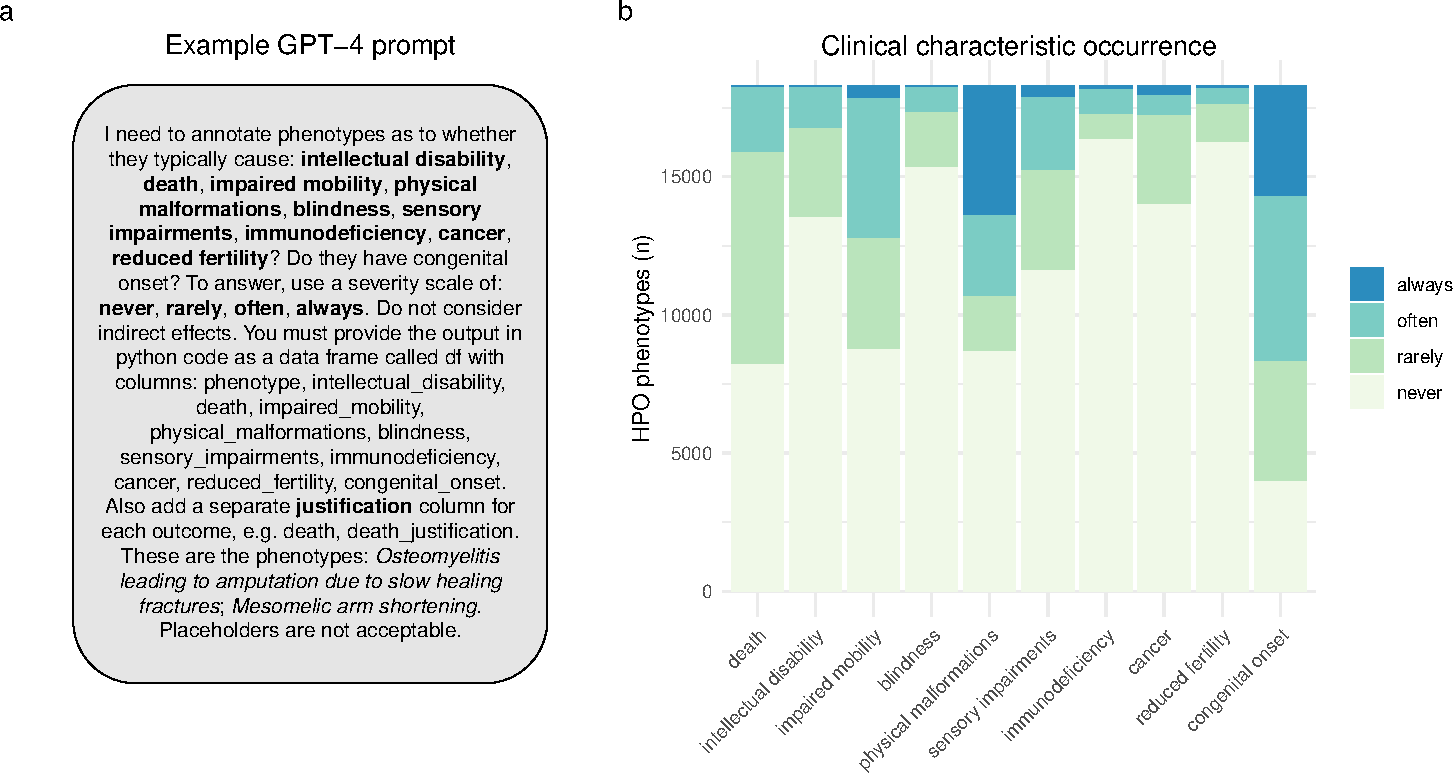
\includegraphics{manuscript_files/figure-pdf/fig-occurrence-1.pdf}

}

\caption{\label{fig-occurrence}GPT-4 was able to annotate all human
phenotypes based on whether they are always/often/rarely/never
associated with different clinical characteristics. \textbf{a}, An
example of the prompt input given to to GPT-4. The phenotypes listed in
the second to last sentence (\emph{italicised}) were changed to allow
all HPO phenotypes to be annotated. \textbf{b}, Stacked bar plot showing
the proportion of the occurrence of each clinical characteristic across
all annotated HPO phenotypes. The terms shown on the x-axis are the
clinical characteristics for which GPT-4 was asked to determine whether
each phenotype caused them.}

\end{figure}%

We employed the OpenAI GPT-4 model with Python to annotate 17502 terms
within the HPO (v2024-02-08) (Gargano et al., 2024; Köhler et al.,
2021). Our annotation framework was developed based on previously
defined criteria for classifying disease severity (Lazarin et al.,
2014). We sought to evaluate the impact of phenotypes on factors
including intellectual disability, death, impaired mobility, physical
malformations, blindness, sensory impairments, immunodeficiency, cancer,
reduced fertility, and congenital onset. Through prompt design we found
that the performance of GPT-4 improved when we incorporated a scale
associated with each effect and required a justification for each
response. For each effect, we asked about the frequency of its
occurrence - whether it never, rarely, often, or always occurred.
Framing the queries in this way served two purposes. First, this helped
to constrain the responses of GPT-4 to a specific range of values,
making answers more consistent and amenable to downstream data analysis.
Second, it served to overcome one of the main limitations noted by
Lazarin et al. (2014) as they did not collect information on how the
frequency of each disease affected their decision making when generating
severity annotations.

Phenotype outcome occurrence varied across annotation categories.
\textgreater50\% of phenotypes never caused blindness, sensory
impairments, immunodeficiency, cancer, reduced fertility or intellectual
disability. Only a minority of phenotypes (21.7\%) never had a
congenital onset, which is expected as rare disorders tend to be early
onset genetic conditions Fig.~\ref{fig-occurrence}.

Less than 1\% of phenotypes always directly resulted in death (n=71),
such as `Stillbirth', `Anencephaly' and `Bilateral lung agenesis'.
Meanwhile, 9707 phenotypes were annotated as often or rarely causing
death. 7880 phenotypes were annotated as never causing death. Examples
of phenotypes that never cause death included 34 unique forms of
syndactyly, a non-lethal condition that causes fused or webbed fingers
(occurring 1 in 1,200--15,000 live births). While not life-threatening
itself, syndactyly is a symptom of genetic disorders that can cause
life-threatening cardiovascular and neurodevelopmental defects, such as
Apert Syndrome (Garagnani \& Smith, 2013). This example highlights the
ability of GPT-4 to successfully distinguish between phenotypes that
directly cause lethality, and those that are often associated with
diseases that cause lethality.

\subsubsection{Annotation consistency and
recall}\label{annotation-consistency-and-recall}

To assess annotation consistency, we queried GPT-4 with a subset of the
HPO phenotypes multiple times (n=793 unique phenotypes). We employed two
different metrics to determine the \emph{consistency rate}. The first,
less stringent metric, defined consistency as the duplicate annotations
being either `always' and `often', or `never' and `rarely'. The second,
more stringent metric, required exact agreement in annotation
occurrences, e.g.~`always' and `always'. For the less stringent metric,
duplicated phenotypes were annotated consistently at a rate of at least
80\%, and for the more stringent metric, the lowest consistency rate was
57\% for congenital onset. An example of where annotations were
inconsistent was for the HPO term `Acute leukaemia'. One time, GPT-4
annotated it as often causing impaired mobility, giving the
justification that `weakness and fatigue from leukaemia and its
treatment can impair mobility'. The other time, GPT-4 annotated it as
rarely causing impaired mobility, giving the justification that `acute
leukaemia rarely impairs mobility directly'. Despite specifying in the
prompt for GPT-4 not to take into consideration indirect effects, this
is an example of where it failed to do so.

We also reasoned that GPT-4 would be better able to give consistent
answers for more specific phenotypes lower in the ontology, as they are
more likely to have a single cause. We found that the stringent
consistency rate did indeed significantly improve with greater HPO
ontology depth (\(X_{Pearson}^2\)=22.17, \(\hat{V}_{Cramer}\)=0.03,
p=0.05). See Figure~\ref{fig-consist-vs-ontLvl} for a visual
representation of this relationship.

\phantomsection\label{cell-fig-checks}
\begin{figure}[H]

\centering{

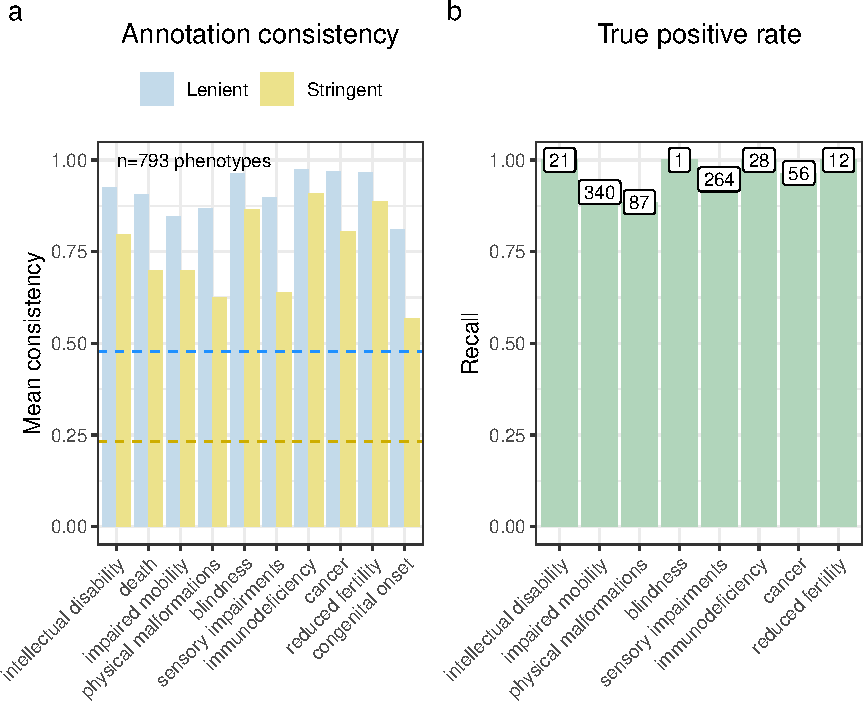
\includegraphics{manuscript_files/figure-pdf/fig-checks-1.pdf}

}

\caption{\label{fig-checks}GPT-4 annotations are consistent and accurate
across annotations. \textbf{a}, Barplot showing the annotation
consistency within phenotypes that were annotated more than once. In the
lenient metric, annotations were collapsed into two groups
(`always'/`often' and `never'/`rarely'). For a given clinical
characteristic within a given phenotype, if an annotation was always
within the same group it was considered consistent. In the stringent
metric, all four annotation categories were considered to be different
from one another. Thus, annotations were only defined as consistent if
they were all identical. The blue dashed line indicates the probability
of two annotations being consistent by chance in the lenient metric
(\textasciitilde1/2). The gold dashed line is the probability of two
annotations being consistent by chance in the stringent metric
(\textasciitilde1/4). \textbf{b}, Bar plot of the true positive rate for
each annotation. The labels above each bar indicate the number of
phenotypes tested.}

\end{figure}%

In order to evaluate the validity of the annotations, we calculated a
true positive rate. This involved identifying specific branches within
the HPO that would contain phenotypes that would reliably indicate the
presence of certain conditions. For instance, the phenotypes `Decreased
fertility in females' and `Decreased fertility in males' should often or
always cause reduced fertility. We observed an encouraging true positive
rate exceeding 88\% across in every clinical characteristic and
achieving perfect recall (100\%) in 4/8 characteristics.

The lowest true positive rate was observed for physical malformations,
with 88.5\% recall across 87 HPO phenotypes. Some cases in which the
GPT-4 annotations disagreed with the HPO ground truth included: `Angioma
serpentinum', `Nevus anemicus', `Pulmonary arteriovenous fistulas'. In
the case of `Angioma serpentinum' it provided the justification that `No
known association with physical malformations'. In another instance,
GPT-4 noted that `Nevus anemicus' is `Limited to hypopigmented skin
patch; no other malformations.'. This indicates that while technically
incorrect according to our predefined benchmarks, a case could in fact
be made that mild skin conditions do not rise to the level of physical
malformations.

This high level of recall underscores the robustness of our annotations
and the reliability of the HPO framework in capturing clinically
relevant phenotypic information. However, we acknowledge that the number
of testable true positive phenotypes for some of these categories are
low, especially `blindness' for which there is only 1 phenotype in the
HPO (after excluding terms pertaining to colour or night blindness).
Furthermore, some of the true positive phenotypes are lexically similar
to the name of the clinical characteristic itself. In these cases,
annotating `Severe intellectual disability' as always causing
intellectual disability is a relatively trivial task. Nevertheless, even
these scenarios provide a clear and interpretable benchmark for the
model's performance. In addition, were numerous phenotypes with
lexically non-obvious relationships to the clinical characteristic that
were annotated correctly by GPT-4. For example, `Molar tooth sign on
MRI' (a neurodevelopmental pathology observed in radiological scans) was
correctly annotated as causing intellectual disability.

\subsubsection{Quantifying phenotypic
severity}\label{quantifying-phenotypic-severity}

While individual annotations are informative, we wanted to be able to
distil the severity of each phenotype into a single score. Quantifying
the overall severity of phenotypes can have important implications for
diagnosis, prognosis, and treatment. It may also guide the
prioritisation of gene therapy trials for phenotypes with the most
severe outcomes and thus the most urgent need. Importantly, the values
reflected the severity of each outcome based on both the type of outcome
itself and its frequency within a particular phenotype. For instance, a
phenotype always causing death would have a higher multiplied value than
a phenotype often causing reduced fertility (see
Table~\ref{tbl-metric-weights}). First, we created a dictionary to map
each phenotype outcome (e.g.~blindness) and its frequency (always,
often, rarely, never) to numeric values from 0-3. Then, the phenotype
outcome values were multiplied by phenotype outcome weights. Next, we
computed an average score for each phenotype by aggregating the
multiplied values across all phenotype outcomes and then calculating the
mean. This was then normalised by the theoretical maximum severity
score, so that all phenotypes were on a 0-100 severity scale (where 100
is the most severe phenotype possible). This average normalised score
represents the overall severity of the phenotype based on the severity
of its individual outcomes.

Based on these scores we evaluated the top 50 severe phenotypes. One of
the most severe phenotype was `Anencephaly' (HP:0002323) with a
composite severity score of 45. Anencephaly is a birth defect where the
baby is born without a portion of its brain and skull, often these
babies are stillborn. In fact, many of the most severe phenotypes were
related to developmental brain and neural tube defects. Comparison of
the severity scores for each response, across the phenotype outcomes
annotated, revealed consistent trends: as the response of the phenotype
outcome increased (from never to always), the severity score also
increased (Supplementary Fig.~\ref{fig-severity-boxplot}). We also
evaluated the severity score distribution by HPO branch and calculated
the mean severity score using all phenotypes within each major HPO
branch (Fig.~\ref{fig-severity-histo}). The HPO branch with the greatest
mean severity score was `Abnormal cellular phenotype' (mean=17),
followed by `Neoplasm' (mean=15.2), which would include the highly
ranked phenotypes seen in Figure~\ref{fig-top-phenos}.

\phantomsection\label{cell-fig-top-phenos}
\begin{figure}[H]

\centering{

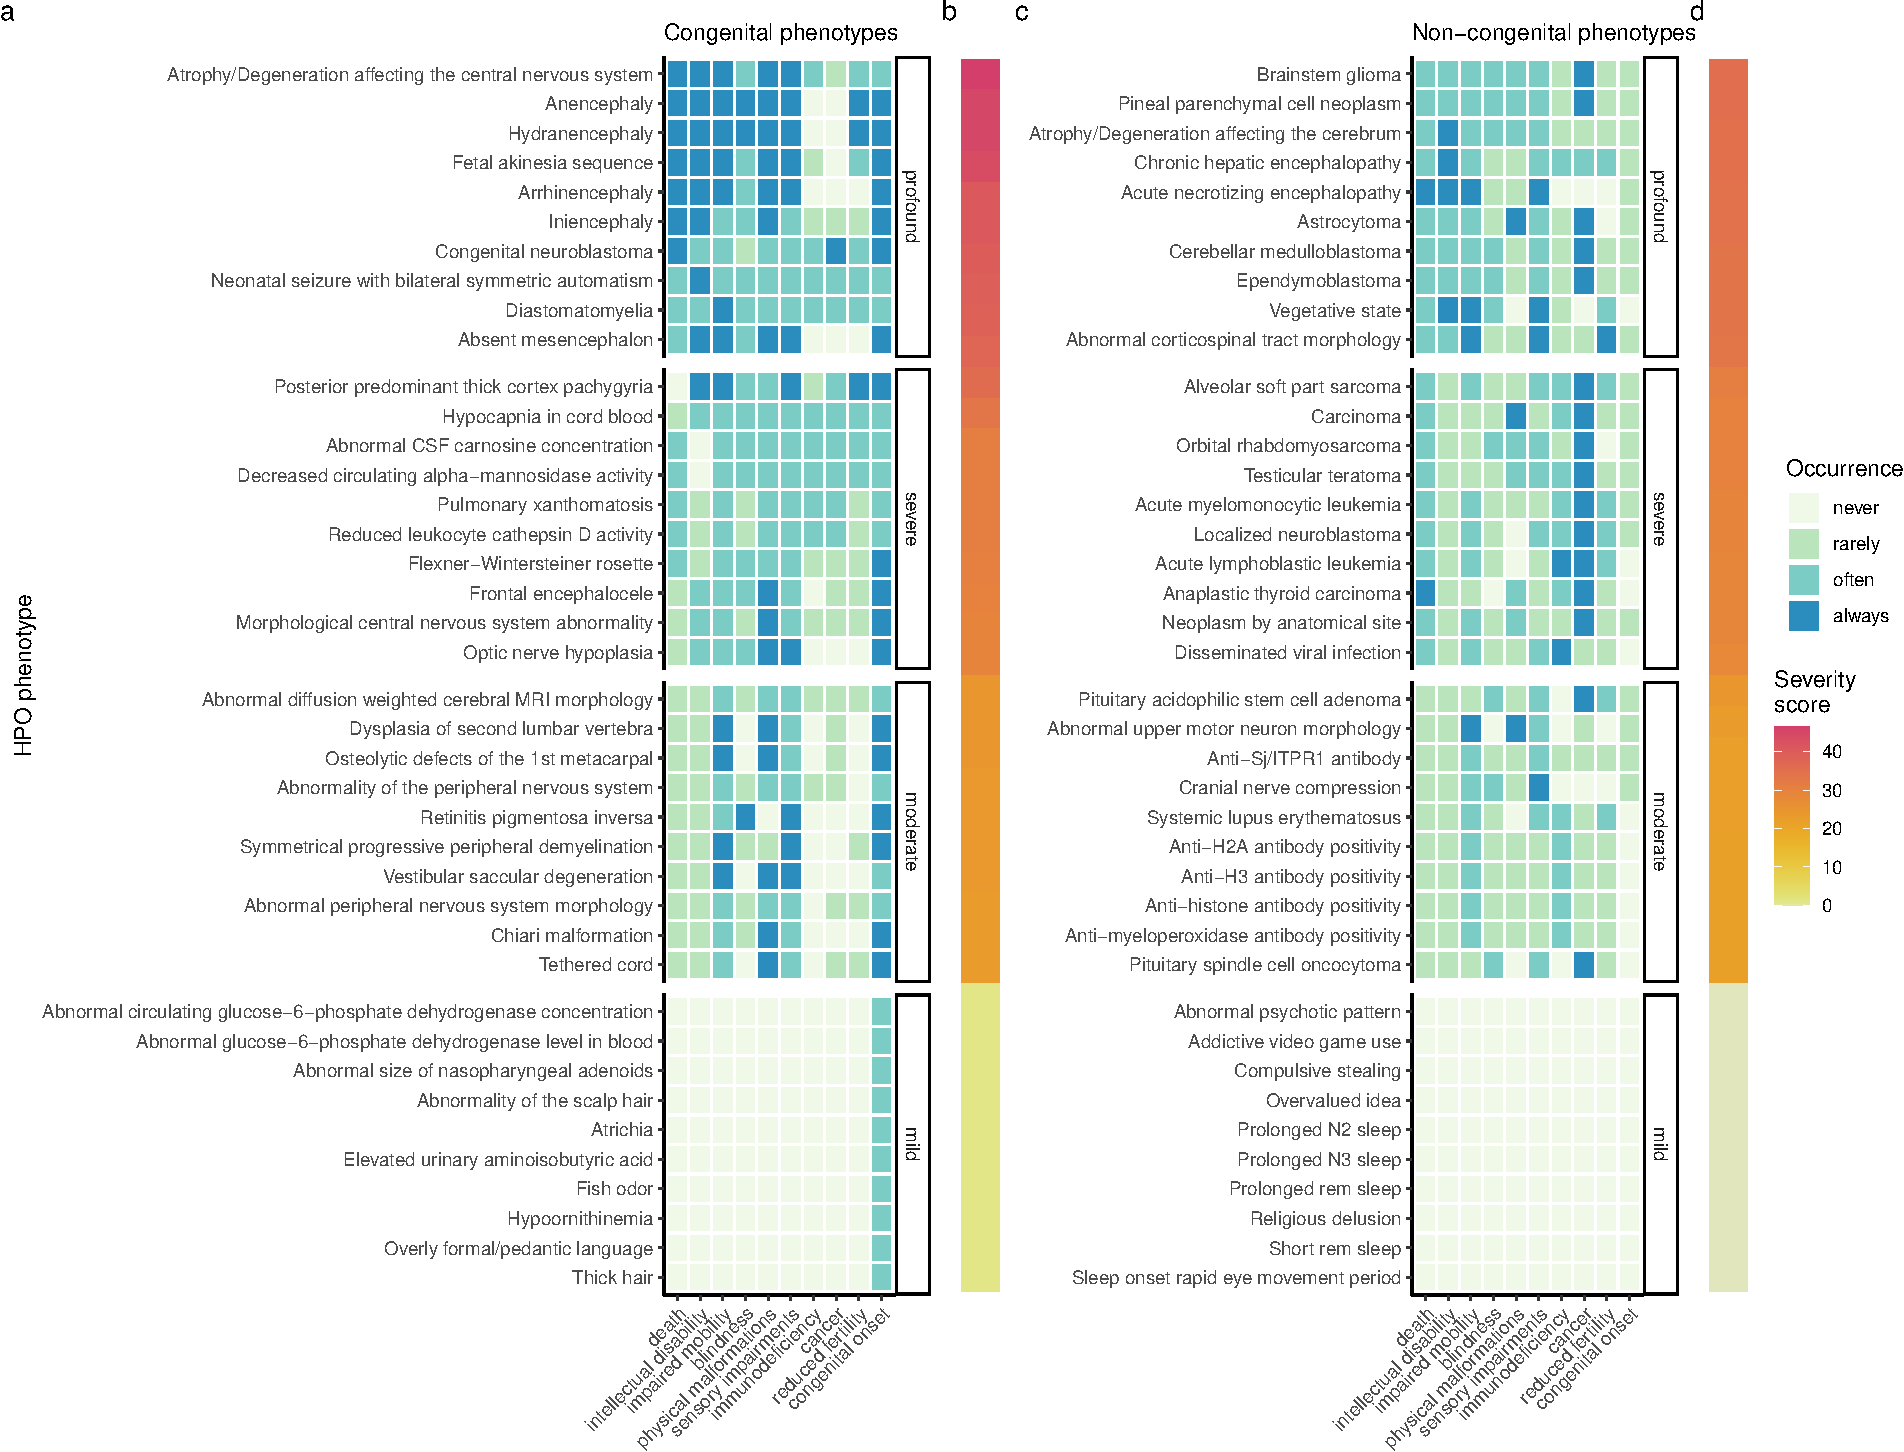
\includegraphics{manuscript_files/figure-pdf/fig-top-phenos-1.pdf}

}

\caption{\label{fig-top-phenos}Quantifying the severity of HPO phenotype
annotations highlights the most impactful conditions. Heatmap of 10
represetantive phenotypes from each severity class (Profound, Severe,
Moderate, Mild) stratified by whether the phenotypes are often/always
congenital (\textbf{a}-\textbf{b}) or rarely/never congenital
(\textbf{c}-\textbf{d}). Continuous severity scores are shown as bars
(\textbf{b},\textbf{d}) and were calculated by multiplying the numeric
values assigned to each clinical characteristic according to
Table~\ref{tbl-metric-weights}. The average normalised score,
representing overall phenotype severity on a 0-100 scale, was calculated
by aggregating the multiplied values and normalising by the theoretical
maximum severity score. The x-axes show each of the clinical
characteristics. All data for this figure, as well as justifications for
each annotation, can be found in Table~\ref{tbl-annotations}.}

\end{figure}%

\subsubsection{Severity classes}\label{severity-classes}

While the continuous severity score is a helpful metric, there may be
some use cases where a categorical classification of severity is more
immediately useful. In work by Lazarin et al. (2014), the authors
defined severity classed using a simple decision tree based on the
individual severity annotations. We approximated this approach using our
GPT-4 annotations. This categorical approach showed a strong degree of
positive correspondence with the continuous severity score
(\(\hat{\omega_{p}^2}\)=0.88, p\textless2.2e-308). In other words,
severity score increased with severity class level (mild \textless{}
moderate \textless{} severe \textless{} profound) as expected. The
distribution of severity classes is shown in
Figure~\ref{fig-severity-class}.

\subsubsection{Correlations between severity
metrics}\label{correlations-between-severity-metrics}

We found that some severity metrics were correlated with one another,
with a mean Pearson correlation of 0.2 across all individual metrics
(see Figure~\ref{fig-metric-corplot}). In particular, blindness and
sensory impairment were highly correlated with one another (r=0.62,
p=0). Some metrics drove the composite severity score more than other,
which is a reflection of both our per-metric weighting scheme, response
type frequencies, and the correlation structure between metrics.
Overall, impaired mobility seemed to be the strongest driver of the
composite severity score with a Pearson correlation of 0.6001824,
followed by intellectual disability (r=0.59) and death (r=0.56).

\subsubsection{Congenital onset by HPO
branch}\label{congenital-onset-by-hpo-branch}

\phantomsection\label{cell-fig-congenital-branches}
\begin{figure}[H]

\centering{

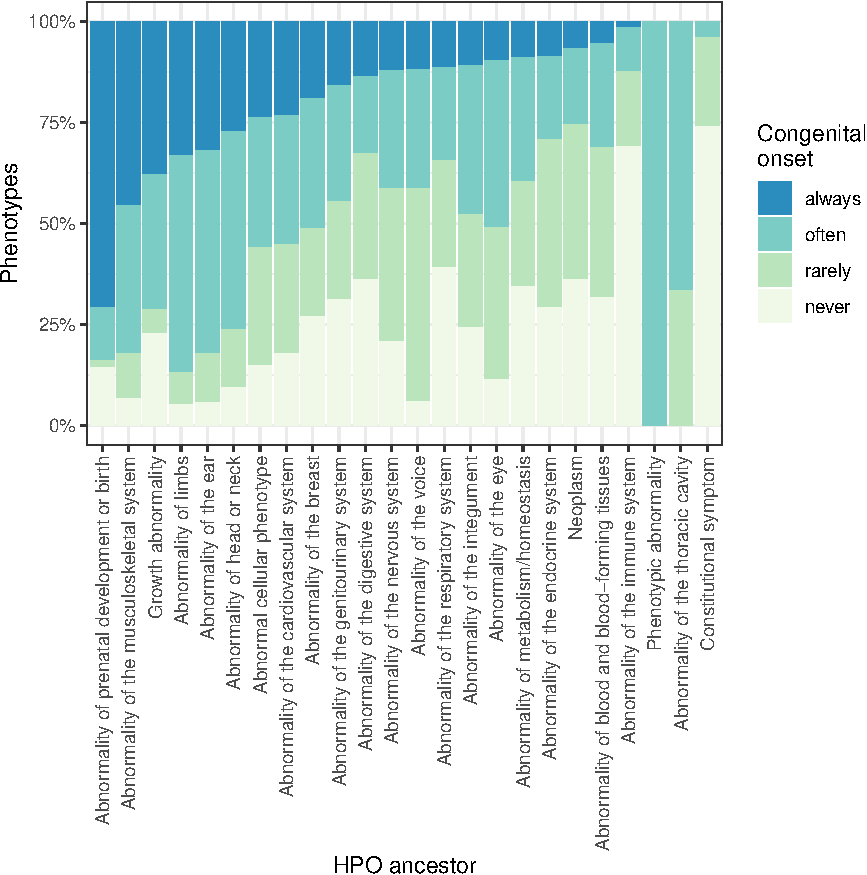
\includegraphics{manuscript_files/figure-pdf/fig-congenital-branches-1.pdf}

}

\caption{\label{fig-congenital-branches}Distribution of congenital onset
across HPO branches. The y-axis shows the proportion of phenotypes that
are always/often/rarely/never congenital. The x-axis shows the HPO
branch, orderered from highest to lowest proportion of always congenital
phenotypes.}

\end{figure}%

Next, we assessed the distribution of congenital onset across HPO
branches (Fig.~\ref{fig-congenital-branches}). We found that the
Abnormality of prenatal development or birth branch contained the
greatest proportion of phenotypes that were always congenital (70.15\%),
followed by Abnormality of the musculoskeletal system (45.34\%) and
Growth abnormality (37.62\%). This is concordant with the expectation
that these phenotypes should largely be congenital. The HPO branches
with the least commonly congenital phenotypes were Constitutional
symptom (0\%), Abnormality of the thoracic cavity (0\%), and Phenotypic
abnormality (0\%).
\href{https://hpo.jax.org/app/browse/term/HP:0025142}{`Constitutional
symptom'} is a fairly broad term defined as \emph{`A symptom or
manifestation indicating a systemic or general effect of a disease and
that may affect the general well-being or status of an individual.'}
Examples include `Fatigue' `Exercise intolerance', `Hot flashes' and
`Sneeze'.

\subsection{Discussion}\label{discussion}

Phenotype severity annotations have utility across a wide variety of
applications in both the clinic and research. In clinical settings,
severity annotations can be used to prioritise the treatment of some
phenotypes over others in patients with complex presentations, avoid
administering contraindicated drugs, and prognosing potential health
outcomes. In research settings, severity annotations can be used to
identify phenotypes that have a large impact on patient outcomes and yet
are currently understudied. They may also be used to help design new
experiments and studies, or even provide new insights into the
underlying aetiology of the disease by making expert-level summaries
more immediately accessible to the wider research community.

The creation and annotation of biomedical knowledge has traditionally
relied on manual or semi-manual curation by human experts (Gargano et
al., 2024; Köhler et al., 2021; Mungall et al., 2017; Ochoa et al.,
2021; Putman et al., 2024). Performing such manual curation and review
tasks at scale is often infeasible for human biomedical experts given
limited time and resources. LLMs have the capacity to effectively
encode, retrieve, and synthesise vast amounts of diverse information in
a highly scalable manner (OpenAI et al., 2024; Singhal, Azizi, et al.,
2023; Van Veen et al., 2024). This makes them powerful tools that can be
applied in a rapidly expanding variety of scenarios, including medical
practice, research and data curation (Caufield et al., 2023; O'Neil et
al., 2024; Pan et al., 2023; Singhal, Azizi, et al., 2023; Toro et al.,
2023).

Here, we introduce a novel framework to leverage the current
best-in-class LLM, GPT-4 (OpenAI et al., 2024), to systematically
annotate the severity of 17502 phenotypic abnormalities within the HPO.
By employing advanced AI capabilities, we have demonstrated the
feasibility of automating this process, significantly enhancing
efficiency without substantially compromising accuracy. Our validation
approach yielded a high true positive rate exceeding 88\% across the
phenotypes tested. Furthermore, our approach can be readily adapted and
scaled to accommodate the growing volume of phenotypic data. In total,
the entire study cost \$296.27 in queries to the OpenAI API. While we do
not have a direct comparison, this likely represents a extremely small
fraction of the total costs of such a study if performed manually by
human experts charging at an hourly rate. Even if all human annotations
were provided on a volunteer basis, this would still require hundreds if
not thousands of hours of cumulative manual human labour. Using our
approach, severity annotations for the entire HPO can be generated
automatically in a matter of several hours.

Throughout this study, we observed that GPT-4 was capable of reliably
recovering deep semantic relationships from the medical domain, far
beyond making superficial inferences based on lexical similarities. An
excellent example of this is the phenotype `Molar tooth sign on MRI'
(HP:0002419; severity score=25.56), which GPT-4 annotated as causing
intellectual disability. At first glance, we ourselves assumed this was
a false positive as the term appeared to be related to dentition.
However, upon further inspection we realised that molar tooth sign is in
fact a pattern of abnormal brain morphology that happens to bear some
resemblance to molar dentition when observed in radiological scans. This
phenotype is a known sign of neurodevelopmental defects that can indeed
cause severe intellectual disability (Gleeson et al., 2004).

In addition to rapidly synthesising and summarising vast amounts of
information, LLMs can also be steered to provide justifications for each
particular response. This makes LLMs amenable to direct interrogation as
a means of recovering explainability, especially when designed to retain
information about previous requests and interactions as they use these
to iteratively improve and update their predictions (Janik, 2024). This
represents a categorical advance over traditional natural language
processing models based on more shallow forms of statistical or machine
learning (e.g.~Term Frequency-Inverse Document Frequency (Jones, 1972),
Word2vec (Mikolov et al., 2013)) which lack the ability to provide
chains of causal reasoning to justify their predictions. This highlights
the fundamental trade-off between simpler models with high
explainability (the ability humans to understand the inner workings of
the model) but low interpretability (the ability of humans to trace the
decision process of the model, analogous to human `reasoning'), and
deeper more complex models with low explainability but high
interpretability (Marcinkevičs \& Vogt, 2023).

A key contribution of our study is the introduction of a quantitative
severity scoring system that integrates both the nature of the phenotype
outcome and the frequency of its occurrence. By encoding the concept of
severity in this way, we are able to prioritise phenotypes based on
their impact on patients. The methodology allowed us to transition from
low-throughput qualitative assessments of severity (e.g. Lazarin et al.
(2014)) to high-throughput quantitative assessments of severity. One of
the most severe phenotypes in the HPO is `Fetal akinesia sequence' (FAS;
HP:0001989, severity score= 43.9), and extremely rare condition that is
almost always lethal. FAS is a complex, multi-system phenotype that can
be caused by at least 24 different genetic disorders. Despite the
complex and heterogeneous aetiology of this phenotype, GPT-4 was able to
provide accurate annotations alongside explainable justifications for
those annotations (see Table~\ref{tbl-fas}). For example, this phenotype
almost always results in death, either \emph{in utero} or shortly after
birth. Not only did GPT-4 correctly provide the annotation death as
`always', when asked whether FAS causes sensory impairments it provided
the response `always' with the justification `Fetal akinesia sequence
typically results in severe sensory impairment due to neurodevelopmental
disruption.' Neurodevelopmental disruption is indeed a hallmark
component of FAS (e.g.~hydrocephalus, cerebellar hypoplasia) that causes
severe impairments across multiple sensory systems (Chen, 2012). This
demonstrates that GPT-4 was able to recover the correct chain of
causality from phenotype to clinical outcome.

Our findings highlight the potential of this next generation of natural
language processing technologies in significantly contributing to the
automation and refinement of data curation in biomedical research. These
results have a large number of useful real-world applications, such as
prioritising gene therapy candidates (Murphy et al., 2023) and guiding
clinical decision-making in rare diseases. It may also be used as tool
to help inform policy decisions and funding allocation by healthcare or
governmental institutions. This of course would need to be in
consultation with subject matter medical experts, patients, advocates
and biomedical ethicists before reaching a final decision. Nevertheless,
access to succinct, interpretable, and semi-quantitative severity
annotations may encourage key decision makers with limited time to
review individual proposals to pay heed to phenotypes and diseases that
would otherwise be overlooked. As the HPO and the broader literature
continue to grow over time, our automated AI-based approach can easily
be repeated to keep pace with the rapidly evolving biomedical landscape.
Furthermore, it can be extended to produce different sets of annotations
or be used with any other ontology. Additional use cases include
gathering data on the prevalence of each phenotype to approximate their
social and financial costs.

One key limitation of our study is the fact that we did not explicitly
interrogate GPT-4 to assess how the availability of treatments affected
the annotations it produced. For example, there are some very severe
conditions for which highly effective treatments and early detection
screens are widely available (e.g.~syphilis, some forms of melanoma),
thus rendering them fully treatable or even curable provided access to
modern healthcare. It would therefore be useful to further interrogate
GPT-4 to uncover how the availability of treatments influences its
responses. Many of our findings here seem to indicate that GPT-4 does
take into account quality of care to the extent that health services
increase the likelihood of desired outcomes. For example, many of the
cancer phenotypes are justified as always or often causing death unless
detected and treated early in the disease course. On the other hand,
some cancers are justified as rarely causing death if appropriate
treatment is provided, which may not always be the case for individuals
or populations with access to less access to quality healthcare
services. Future efforts could more explicitly ask GPT-4 whether the
phenotype would cause death with no or suboptimal treatment.

Another limitation with the present dataset is that phenotypes
themselves can manifest with different degrees of severity, in the sense
that they are more pronounced or intense. For example, sensitivity to
light could range from a mild inconvenience to a severe disability that
prevents the individual from leaving their home during the day. The
effect of onset (beyond congenital vs.~non-congenital) and time course
(acute, slowly progression, relapse-remitting) were also not explicitly
considered. Finally, we did not ask GPT-4 to consider phenotypes as they
present within particular diseases. For example, while the phenotype
`Hypertension' may be mild to moderate in the general population and not
present until middle-age, it can also present early in life as very
severe in the context of a rare genetic disorder such as Liddle
syndrome. Future work could explore these nuances in more detail.

In addition to these technical challenges, there are multiple factors
that need to be considered when trying to prioritise phenotypes for
their suitability for gene therapy development. First, while we have
attempted to formalise severity here, this is an inherently subjective
concept that may vary considerably across different individuals and
contexts. For instance, one could ask whether a condition that always
causes death is worse than a condition that causes a lifetime of severe
disability (e.g.~paralysis, blindness, intellectual disability). Metrics
such as quality-adjusted life years (QALYs) have been proposed in the
past to address these dilemmas by defining health as a function of both
the length and quality of life (Prieto \& Sacristán, 2003). With regards
to the financial burden of diseases, in some situations phenotypes which
require many years of expensive medical care may be prioritised over
those that result in extremely early onset lethality and little
opportunity for therapeutic intervention. Another factor that affects
the viability of a therapeutic program is the speed, cost and other
practical considerations of a clinical trial. For instance, measuring
risk of ageing-related respiratory failure over a ten-year period may be
impractical in some cases. However, testing for total reversal of an
existing severe phenotype could potentially yield faster and more
immediately impactful results. If performed in close collaboration with
medical ethicists, governmental organisations, advocacy groups and
patient families, such cost/benefit assessments could be aided by LLMs
through the scalable gathering of relevant data. As AI capabilities
continue to advance, the range of applications in which they can be used
effectively will continue to grow.

While our study demonstrates the feasibility and utility of AI-driven
phenotypic annotation, several limitations must be acknowledged. The
reliance on computational algorithms may introduce biases or
inaccuracies inherent to the training data, necessitating ongoing
validation and refinement of our approach. Additionally, our severity
scoring system, while comprehensive, may not capture the full spectrum
of phenotypic variability or account for complex gene-environment
interactions. Future research should focus on further optimising
AI-driven annotation methodologies, incorporating additional data
modalities such as genomic and clinical data to enhance accuracy.

In conclusion, our study represents a significant step towards
harnessing the power of AI to advance phenotypic annotation and severity
assessment across all rare diseases. This resource aims to provide
researchers and clinicians with actionable insights that can inform rare
disease research and improve the lives of individuals affected by rare
diseases.

\subsection{Methods}\label{methods}

\subsubsection{Annotating the HPO using OpenAI
GPT-4}\label{annotating-the-hpo-using-openai-gpt-4}

We wrote a Python script to iteratively query GPT-4 via the OpenAI
application programming interface (API). The ultimately yielded
consistently formatted annotations for 17502 terms within the HPO. Our
annotation framework was developed based on previously defined criteria
for classifying disease severity (Lazarin et al., 2014). We sought to
evaluate whether each phenotype directly caused a given severity-related
clinical characteristic, including: intellectual disability, death,
impaired mobility, physical malformations, blindness, sensory
impairments, immunodeficiency, cancer, reduced fertility, and/or had a
congenital onset. Through prompt engineering we found that the
performance of GPT-4 improved when we incorporated a scale associated
with each effect and required a justification for each response. We
asked how frequently the given phenotype directly causes each clinical
characteristic - whether it never, rarely, often, or always occurred.
This design helps to constrain the potential responses of GPT-4 and thus
make it more amenable to machine-readable post-processing. It also
serves to address one of its key limitations from the Lazarin et al.
(2014) survey, namely the lack information on how clinical
characteristic frequency affected the clinicians' severity annotations.
Here, we can instead use the frequency values to generate more precise
annotations and downstream severity ranking scores.

Furthermore, our prompt design revealed that the optimal trade-off
between the number of phenotypes and performance (in terms of producing
the desired annotations, and adhering to the formatting requirements)
was achieved when inputting no more than two or three phenotypes per
prompt. An example prompt can be seen in Figure~\ref{fig-occurrence}.
Thus, only two phenotypes were included per prompt in order to 1) avoid
exceeding per-query token limits, and 2) prevent the breakdown of GPT-4
performance due to long-form text input, which is presently a known
limitation common to many LLMs including GPT-4 (Wei et al., 2024).

\subsubsection{Calculating the true positive
rate}\label{calculating-the-true-positive-rate}

\begin{longtable}[]{@{}
  >{\raggedright\arraybackslash}p{(\columnwidth - 4\tabcolsep) * \real{0.4000}}
  >{\raggedright\arraybackslash}p{(\columnwidth - 4\tabcolsep) * \real{0.4000}}
  >{\raggedleft\arraybackslash}p{(\columnwidth - 4\tabcolsep) * \real{0.2000}}@{}}

\caption{\label{tbl-true-positives}For each clinical characteristic, any
terms that matched}

\tabularnewline

\toprule\noalign{}
\begin{minipage}[b]{\linewidth}\raggedright
Clinical characteristic
\end{minipage} & \begin{minipage}[b]{\linewidth}\raggedright
HPO queries
\end{minipage} & \begin{minipage}[b]{\linewidth}\raggedleft
True positive HPO IDs
\end{minipage} \\
\midrule\noalign{}
\endhead
\bottomrule\noalign{}
\endlastfoot
Intellectual disability & `Intellectual disability'; `Mental
deterioration' & 19 \\
Impaired mobility & `Gait disturbance'; `Diminished movement'; '
mobility' & 319 \\
Physical malformations & `malformation' & 78 \\
Blindness & `blindness' & 1 \\
Sensory impairments & `Abnormality of vision'; `Abnormality of the sense
of smell'; `Abnormality of taste sensation'; `Somatic sensory
dysfunction'; `Hearing abnormality' & 252 \\
Immunodeficiency & `Immunodeficiency'; `Impaired antigen-specific
response' & 29 \\
Cancer & `Cancer'; `malignant'; `carcinoma' & 56 \\
Reduced fertility & `Decreased fertility'; `Hypogonadism' & 9 \\

\end{longtable}

A true positive rate was calculated as a measure of the recall of the
GPT-4 annotations. This was achieved by identifying specific branches
within the HPO that would contain phenotypes that would reliably
indicate the occurrence of certain clinical characteristics, and using
all descendants of this HPO branch as true positives. For example, all
descendants of the terms `Intellectual disability' (HP:0001249) or
`Mental deterioration' (HP:0001268) should be annotated as always or
often causing intellectual disability (Table~\ref{tbl-true-positives}).

\subsubsection{Quantifying phenotypic
severity}\label{quantifying-phenotypic-severity-1}

The GPT-4 generated annotation occurrences were converted into a
semi-quantitative scoring system, with `always' corresponding to 3,
`often' to 2, `rarely' to 1, and `never' to 0. These scores were then
weighted by a severity metric on a scale of 1-5, with 5 representing the
highest severity, as determined by the provided annotations
(Table~\ref{tbl-metric-weights}). Subsequently, the weighted scores
underwent normalisation to yield a final quantitative severity score
ranging from 0-100, with 100 signifying the maximum severity score
attainable.

Let us denote:

\begin{itemize}
\item
  \(p\) : a phenotype in the HPO.
\item
  \(j\) : the identity of a given annotation metric (i.e.~clinical
  characteristic, such as `intellectual disability' or `congenital
  onset').
\item
  \(W_j\): the assigned weight of metric \(j\).
\item
  \(F_j\): the maximum possible value for metric \(j\) (equivalent
  across all \(j\)).
\item
  \(F_{pj}\) : the numerically encoded value of annotation metric \(j\)
  for phenotype \(p\).
\item
  \(NSS_p\): the final composite severity score for phenotype \(p\)
  after applying normalisation to align values to a 0-100 scale and
  ensure equivalent meaning regardless of which other phenotypes are
  being analysed in addition to \(p\). This allows for direct
  comparability of severity scores across studies with different sets of
  phenotypes.
\end{itemize}

\hfill\break
\hfill\break

\begin{equation*}
  \eqnmarkbox[Brown4]{nss}{NSS_p}
  =
  \frac{ 
    \eqnmarkbox[Goldenrod]{nss2}{\sum_{j=1}^{m}} 
    (
      \eqnmarkbox[Goldenrod4]{nss3}{F_{pj}}
      \times 
      \eqnmarkbox[IndianRed4]{nss4}{W_j}
    )
    }{
    \eqnmarkbox[Tan]{nss5}{\sum_{j=1}^{m}(\max\{F_j\} \times W_j)} 
  } \times 100
\end{equation*}
\annotate[yshift=1em]{left}{nss}{Normalised Severity Score \\for each phenotype}
\annotate[yshift=3em]{left}{nss2}{Sum of weighted annotation values \\across all metrics}
\annotate[yshift=3em]{right}{nss3}{Numerically encoded annotation value \\of metric $j$ for phenotype $p$}
\annotate[yshift=1em]{right}{nss4}{Weight for metric $j$} 
\annotate[yshift=-1em]{below,right}{nss5}{Theoretical maximum severity score}

\hfill\break

\begin{longtable}[]{@{}
  >{\raggedright\arraybackslash}p{(\columnwidth - 8\tabcolsep) * \real{0.4000}}
  >{\raggedleft\arraybackslash}p{(\columnwidth - 8\tabcolsep) * \real{0.1571}}
  >{\raggedleft\arraybackslash}p{(\columnwidth - 8\tabcolsep) * \real{0.1429}}
  >{\raggedleft\arraybackslash}p{(\columnwidth - 8\tabcolsep) * \real{0.1571}}
  >{\raggedleft\arraybackslash}p{(\columnwidth - 8\tabcolsep) * \real{0.1429}}@{}}

\caption{\label{tbl-metric-weights}Weighted scores for each clinical
characteristic and GPT-4 response category.}

\tabularnewline

\toprule\noalign{}
\begin{minipage}[b]{\linewidth}\raggedright
Clinical characteristic
\end{minipage} & \begin{minipage}[b]{\linewidth}\raggedleft
Always (3)
\end{minipage} & \begin{minipage}[b]{\linewidth}\raggedleft
Often (2)
\end{minipage} & \begin{minipage}[b]{\linewidth}\raggedleft
Rarely (1)
\end{minipage} & \begin{minipage}[b]{\linewidth}\raggedleft
Never (0)
\end{minipage} \\
\midrule\noalign{}
\endhead
\bottomrule\noalign{}
\endlastfoot
Death (6) & 18 & 12 & 6 & 0 \\
Intellectual disability (5) & 15 & 10 & 5 & 0 \\
Impaired mobility (4) & 12 & 8 & 4 & 0 \\
Blindness (4) & 12 & 8 & 4 & 0 \\
Physical malformations (3) & 9 & 6 & 3 & 0 \\
Sensory impairments (3) & 9 & 6 & 3 & 0 \\
Immunodeficiency (3) & 9 & 6 & 3 & 0 \\
Cancer (3) & 9 & 6 & 3 & 0 \\
Reduced fertility (1) & 3 & 2 & 1 & 0 \\
Congenital onset (1) & 3 & 2 & 1 & 0 \\

\end{longtable}

\subsubsection{Severity classes}\label{severity-classes-1}

The decision tree algorithm used in Lazarin et al. (2014) was adapted
here for use with the GPT-4 annotations. This algorithm first assigned
each annotation metric to a tier, where Tier 1 indicated the most severe
annotation metrics and Tier 4 indicated the least severe annotation
metrics (`death'=1, `intellectual disability'=1, `impaired mobility'=2,
`physical malformations'=2, `blindness'=3, `sensory impairments'=3,
`immunodeficiency'=3, `cancer'=3, `reduced fertility'=4). If a phenotype
often or always caused more than one Tier 1 annotation, it was assigned
a severity class of ``Profound''. If the phenotype often or always
caused only one Tier 1 annotation, it was assigned a severity class of
``Severe''. A ``Severe'' class assignment was also assigned if the
phenotype often or always caused three or more Tier 2 and Tier3
annotations. If the phenotype often or always caused at least one Tier 2
annotation, it was assigned a severity class of ``Moderate''. All
remaining phenotypes were was assigned a severity class of ``Mild''. In
cases where the phenotype mapped to more than one class, only the most
severe class was used. This procedure is implemented within the function
\texttt{HPOExplorer::gpt\_annot\_class}.

\subsubsection{Correlations between severity
metrics}\label{correlations-between-severity-metrics-1}

To assess the correlation structure between each severity metric, as
well as between the composite severity score and each metric, we
computed Pearson correlation coefficients for all pairwise combinations
of these variables using the numerically encoded metric values. The
correlation matrix was visualised using a heatmap, with the colour
intensity representing the strength of the correlation
(Figure~\ref{fig-metric-corplot}).

\subsection{Data and code availability
statement}\label{data-and-code-availability-statement}

All code and data used in this study are available on GitHub at:

\url{https://github.com/neurogenomics/gpt_hpo_annotations}

The GPT-4 annotations for all HPO phenotypes are made available through
the R function \texttt{HPOExplorer::gpt\_annot\_read} or in CSV format
at:

\url{https://github.com/neurogenomics/gpt_hpo_annotations/tree/master/data}

A fully reproducible version of this Quarto manuscript can be found at:

\url{https://github.com/neurogenomics/gpt_hpo_annotations/blob/master/manuscript.qmd}

\subsection{Acknowledgements}\label{acknowledgements}

We would like to thank members of the Monarch Initiative for their
insight and feedback throughout this project. In particular, Peter
Robinson.

\subsubsection{Funding}\label{funding}

This work was supported by a UK Dementia Research Institute (UK DRI)
Future Leaders Fellowship {[}MR/T04327X/1{]} and the UK DRI which
receives its funding from UK DRI Ltd, funded by the UK Medical Research
Council, Alzheimer's Society and Alzheimer's Research UK.

\subsection*{References}\label{references}
\addcontentsline{toc}{subsection}{References}

\phantomsection\label{refs}
\begin{CSLReferences}{1}{0}
\vspace{1em}

\bibitem[\citeproctext]{ref-boltonBioMedLM7BParameter2024}
Bolton, E., Venigalla, A., Yasunaga, M., Hall, D., Xiong, B., Lee, T.,
et al. (2024). BioMedLM: A 2.7B parameter language model trained on
biomedical text. \emph{arXiv}.
\url{https://doi.org/10.48550/arXiv.2403.18421}

\bibitem[\citeproctext]{ref-caufieldStructuredPromptInterrogation2023}
Caufield, J. H., Hegde, H., Emonet, V., Harris, N. L., Joachimiak, M.
P., Matentzoglu, N., et al. (2023). Structured prompt interrogation and
recursive extraction of semantics (SPIRES): A method for populating
knowledge bases using zero-shot learning. \emph{arXiv}.
\url{https://doi.org/10.48550/arXiv.2304.02711}

\bibitem[\citeproctext]{ref-chenPrenatalDiagnosisGenetic2012}
Chen, C.-P. (2012). Prenatal diagnosis and genetic analysis of fetal
akinesia deformation sequence and multiple pterygium syndrome associated
with neuromuscular junction disorders: A review. \emph{Taiwanese Journal
of Obstetrics and Gynecology}, \emph{51}(1), 12--17.
\url{https://doi.org/10.1016/j.tjog.2012.01.004}

\bibitem[\citeproctext]{ref-chengExploringPotentialGPT42023}
Cheng, K., Guo, Q., He, Y., Lu, Y., Gu, S., \& Wu, H. (2023). Exploring
the potential of GPT-4 in biomedical engineering: The dawn of a new era.
\emph{Annals of Biomedical Engineering}, \emph{51}(8), 1645--1653.
\url{https://doi.org/10.1007/s10439-023-03221-1}

\bibitem[\citeproctext]{ref-garagnaniSyndromesAssociatedSyndactyly2013}
Garagnani, L., \& Smith, G. D. (2013). Syndromes associated with
syndactyly. In J. M. Abzug, S. Kozin, \& D. A. Zlotolow (Eds.),
\emph{The pediatric upper extremity} (pp. 1--31). Springer.
\url{https://doi.org/10.1007/978-1-4614-8758-6_14-1}

\bibitem[\citeproctext]{ref-garganoHumanPhenotypeOntology2024}
Gargano, M. A., Matentzoglu, N., Coleman, B., Addo-Lartey, E. B.,
Anagnostopoulos, A. V., Anderton, J., et al. (2024). The human phenotype
ontology in 2024: Phenotypes around the world. \emph{Nucleic Acids
Research}, \emph{52}(D1), D1333--D1346.
\url{https://doi.org/10.1093/nar/gkad1005}

\bibitem[\citeproctext]{ref-gleesonMolarToothSign2004}
Gleeson, J. G., Keeler, L. C., Parisi, M. A., Marsh, S. E., Chance, P.
F., Glass, I. A., et al. (2004). Molar tooth sign of the
midbrain--hindbrain junction: Occurrence in multiple distinct syndromes.
\emph{American Journal of Medical Genetics Part A}, \emph{125A}(2),
125--134. \url{https://doi.org/10.1002/ajmg.a.20437}

\bibitem[\citeproctext]{ref-guDomainSpecificLanguageModel2021}
Gu, Y., Tinn, R., Cheng, H., Lucas, M., Usuyama, N., Liu, X., et al.
(2021). Domain-specific language model pretraining for biomedical
natural language processing. \emph{ACM Transactions on Computing for
Healthcare}, \emph{3}(1), 2:1--2:23.
\url{https://doi.org/10.1145/3458754}

\bibitem[\citeproctext]{ref-janikAspectsHumanMemory2024}
Janik, R. A. (2024). Aspects of human memory and large language models.
\emph{arXiv}. \url{https://doi.org/10.48550/arXiv.2311.03839}

\bibitem[\citeproctext]{ref-jonesStatisticalInterpretationTerm1972}
Jones, K. S. (1972). A statistical interpretation of term specificity
and its application in retrieval. \emph{Journal of Documentation},
\emph{28}(1), 11--21. \url{https://doi.org/10.1108/eb026526}

\bibitem[\citeproctext]{ref-kohlerHumanPhenotypeOntology2021}
Köhler, S., Gargano, M., Matentzoglu, N., Carmody, L. C., Lewis-Smith,
D., Vasilevsky, N. A., et al. (2021). The human phenotype ontology in
2021. \emph{Nucleic Acids Research}, \emph{49}(D1), D1207--D1217.
\url{https://doi.org/10.1093/nar/gkaa1043}

\bibitem[\citeproctext]{ref-labrakBioMistralCollectionOpenSource2024}
Labrak, Y., Bazoge, A., Morin, E., Gourraud, P.-A., Rouvier, M., \&
Dufour, R. (2024). BioMistral: A collection of open-source pretrained
large language models for medical domains. \emph{arXiv}.
\url{https://doi.org/10.48550/arXiv.2402.10373}

\bibitem[\citeproctext]{ref-Lazarin2014-rz}
Lazarin, G. A., Hawthorne, F., Collins, N. S., Platt, E. A., Evans, E.
A., \& Haque, I. S. (2014). Systematic classification of disease
severity for evaluation of expanded carrier screening panels. \emph{PLoS
One}, \emph{9}(12), e114391.

\bibitem[\citeproctext]{ref-luoBioGPTGenerativePretrained2022}
Luo, R., Sun, L., Xia, Y., Qin, T., Zhang, S., Poon, H., \& Liu, T.-Y.
(2022). BioGPT: Generative pre-trained transformer for biomedical text
generation and mining. \emph{Briefings in Bioinformatics}, \emph{23}(6),
bbac409. \url{https://doi.org/10.1093/bib/bbac409}

\bibitem[\citeproctext]{ref-marcinkevicsInterpretabilityExplainabilityMachine2023}
Marcinkevičs, R., \& Vogt, J. E. (2023). Interpretability and
explainability: A machine learning zoo mini-tour. \emph{arXiv}.
\url{https://doi.org/10.48550/arXiv.2012.01805}

\bibitem[\citeproctext]{ref-mcduffAccurateDifferentialDiagnosis2023}
McDuff, D., Schaekermann, M., Tu, T., Palepu, A., Wang, A., Garrison,
J., et al. (2023). Towards accurate differential diagnosis with large
language models. \emph{arXiv}.
\url{https://doi.org/10.48550/arXiv.2312.00164}

\bibitem[\citeproctext]{ref-mikolovEfficientEstimationWord2013}
Mikolov, T., Chen, K., Corrado, G., \& Dean, J. (2013). Efficient
estimation of word representations in vector space. \emph{arXiv}.
\url{https://doi.org/10.48550/arXiv.1301.3781}

\bibitem[\citeproctext]{ref-mungallMonarchInitiativeIntegrative2017a}
Mungall, C. J., McMurry, J. A., Köhler, S., Balhoff, J. P., Borromeo,
C., Brush, M., et al. (2017). The monarch initiative: An integrative
data and analytic platform connecting phenotypes to genotypes across
species. \emph{Nucleic Acids Research}, \emph{45}(D1), D712--D722.
\url{https://doi.org/10.1093/nar/gkw1128}

\bibitem[\citeproctext]{ref-murphyIdentificationCellTypespecific2023}
Murphy, K. B., Gordon-Smith, R., Chapman, J., Otani, M., Schilder, B.
M., \& Skene, N. G. (2023). Identification of cell type-specific gene
targets underlying thousands of rare diseases and subtraits.
\emph{medRxiv}. \url{https://doi.org/10.1101/2023.02.13.23285820}

\bibitem[\citeproctext]{ref-noriCanGeneralistFoundation2023}
Nori, H., Lee, Y. T., Zhang, S., Carignan, D., Edgar, R., Fusi, N., et
al. (2023). Can generalist foundation models outcompete special-purpose
tuning? Case study in medicine. \emph{arXiv}.
\url{https://doi.org/10.48550/arXiv.2311.16452}

\bibitem[\citeproctext]{ref-oneilPhenomicsAssistantInterface2024}
O'Neil, S. T., Schaper, K., Elsarboukh, G., Reese, J. T., Moxon, S. A.
T., Harris, N. L., et al. (2024). Phenomics assistant: An interface for
LLM-based biomedical knowledge graph exploration. \emph{bioRxiv}.
\url{https://doi.org/10.1101/2024.01.31.578275}

\bibitem[\citeproctext]{ref-ochoaOpenTargetsPlatform2021}
Ochoa, D., Hercules, A., Carmona, M., Suveges, D., Gonzalez-Uriarte, A.,
Malangone, C., et al. (2021). Open targets platform: Supporting
systematic drug--target identification and prioritisation. \emph{Nucleic
Acids Research}, \emph{49}(D1), D1302--D1310.
\url{https://doi.org/10.1093/nar/gkaa1027}

\bibitem[\citeproctext]{ref-openaiGPT4TechnicalReport2024}
OpenAI, Achiam, J., Adler, S., Agarwal, S., Ahmad, L., Akkaya, I., et
al. (2024). GPT-4 technical report. \emph{arXiv}.
\url{https://doi.org/10.48550/arXiv.2303.08774}

\bibitem[\citeproctext]{ref-panLargeLanguageModels2023}
Pan, J. Z., Razniewski, S., Kalo, J.-C., Singhania, S., Chen, J.,
Dietze, S., et al. (2023). Large language models and knowledge graphs:
Opportunities and challenges. \emph{arXiv}.
\url{https://doi.org/10.48550/arXiv.2308.06374}

\bibitem[\citeproctext]{ref-prietoProblemsSolutionsCalculating2003}
Prieto, L., \& Sacristán, J. A. (2003). Problems and solutions in
calculating quality-adjusted life years (QALYs). \emph{Health and
Quality of Life Outcomes}, \emph{1}, 80.
\url{https://doi.org/10.1186/1477-7525-1-80}

\bibitem[\citeproctext]{ref-putmanMonarchInitiative20242024}
Putman, T. E., Schaper, K., Matentzoglu, N., Rubinetti, V. P.,
Alquaddoomi, F. S., Cox, C., et al. (2024). The monarch initiative in
2024: An analytic platform integrating phenotypes, genes~and diseases
across species. \emph{Nucleic Acids Research}, \emph{52}(D1),
D938--D949. \url{https://doi.org/10.1093/nar/gkad1082}

\bibitem[\citeproctext]{ref-shinBioMegatronLargerBiomedical2020}
Shin, H.-C., Zhang, Y., Bakhturina, E., Puri, R., Patwary, M., Shoeybi,
M., \& Mani, R. (2020). BioMegatron: Larger biomedical domain language
model. In B. Webber, T. Cohn, Y. He, \& Y. Liu (Eds.), \emph{Proceedings
of the 2020 conference on empirical methods in natural language
processing (EMNLP)} (pp. 4700--4706). Association for Computational
Linguistics. \url{https://doi.org/10.18653/v1/2020.emnlp-main.379}

\bibitem[\citeproctext]{ref-singhalLargeLanguageModels2023}
Singhal, K., Azizi, S., Tu, T., Mahdavi, S. S., Wei, J., Chung, H. W.,
et al. (2023). Large language models encode clinical knowledge.
\emph{Nature}, 1--9. \url{https://doi.org/10.1038/s41586-023-06291-2}

\bibitem[\citeproctext]{ref-singhalExpertLevelMedicalQuestion2023}
Singhal, K., Tu, T., Gottweis, J., Sayres, R., Wulczyn, E., Hou, L., et
al. (2023). Towards expert-level medical question answering with large
language models. \emph{arXiv}.
\url{https://doi.org/10.48550/arXiv.2305.09617}

\bibitem[\citeproctext]{ref-toroDynamicRetrievalAugmented2023}
Toro, S., Anagnostopoulos, A. V., Bello, S., Blumberg, K., Cameron, R.,
Carmody, L., et al. (2023). Dynamic retrieval augmented generation of
ontologies using artificial intelligence (DRAGON-AI). \emph{arXiv}.
\url{https://doi.org/10.48550/arXiv.2312.10904}

\bibitem[\citeproctext]{ref-vanveenAdaptedLargeLanguage2024}
Van Veen, D., Van Uden, C., Blankemeier, L., Delbrouck, J.-B., Aali, A.,
Bluethgen, C., et al. (2024). Adapted large language models can
outperform medical experts in clinical text summarization. \emph{Nature
Medicine}, 1--9. \url{https://doi.org/10.1038/s41591-024-02855-5}

\bibitem[\citeproctext]{ref-weiLongformFactualityLarge2024}
Wei, J., Yang, C., Song, X., Lu, Y., Hu, N., Huang, J., et al. (2024).
Long-form factuality in large language models. \emph{arXiv}. Retrieved
from \url{http://arxiv.org/abs/2403.18802}

\bibitem[\citeproctext]{ref-zhangBiomedGPTUnifiedGeneralist2023}
Zhang, K., Yu, J., Yan, Z., Liu, Y., Adhikarla, E., Fu, S., et al.
(2023). BiomedGPT: A unified and generalist biomedical generative
pre-trained transformer for vision, language, and multimodal tasks.
\emph{arXiv}. \url{https://doi.org/10.48550/arXiv.2305.17100}

\end{CSLReferences}

\newpage{}

\subsection{Supplementary Materials}\label{supplementary-materials}

\subsubsection{Supplementary Figures}\label{supplementary-figures}

\phantomsection\label{cell-fig-consist-vs-ontLvl}
\begin{figure}[H]

\centering{

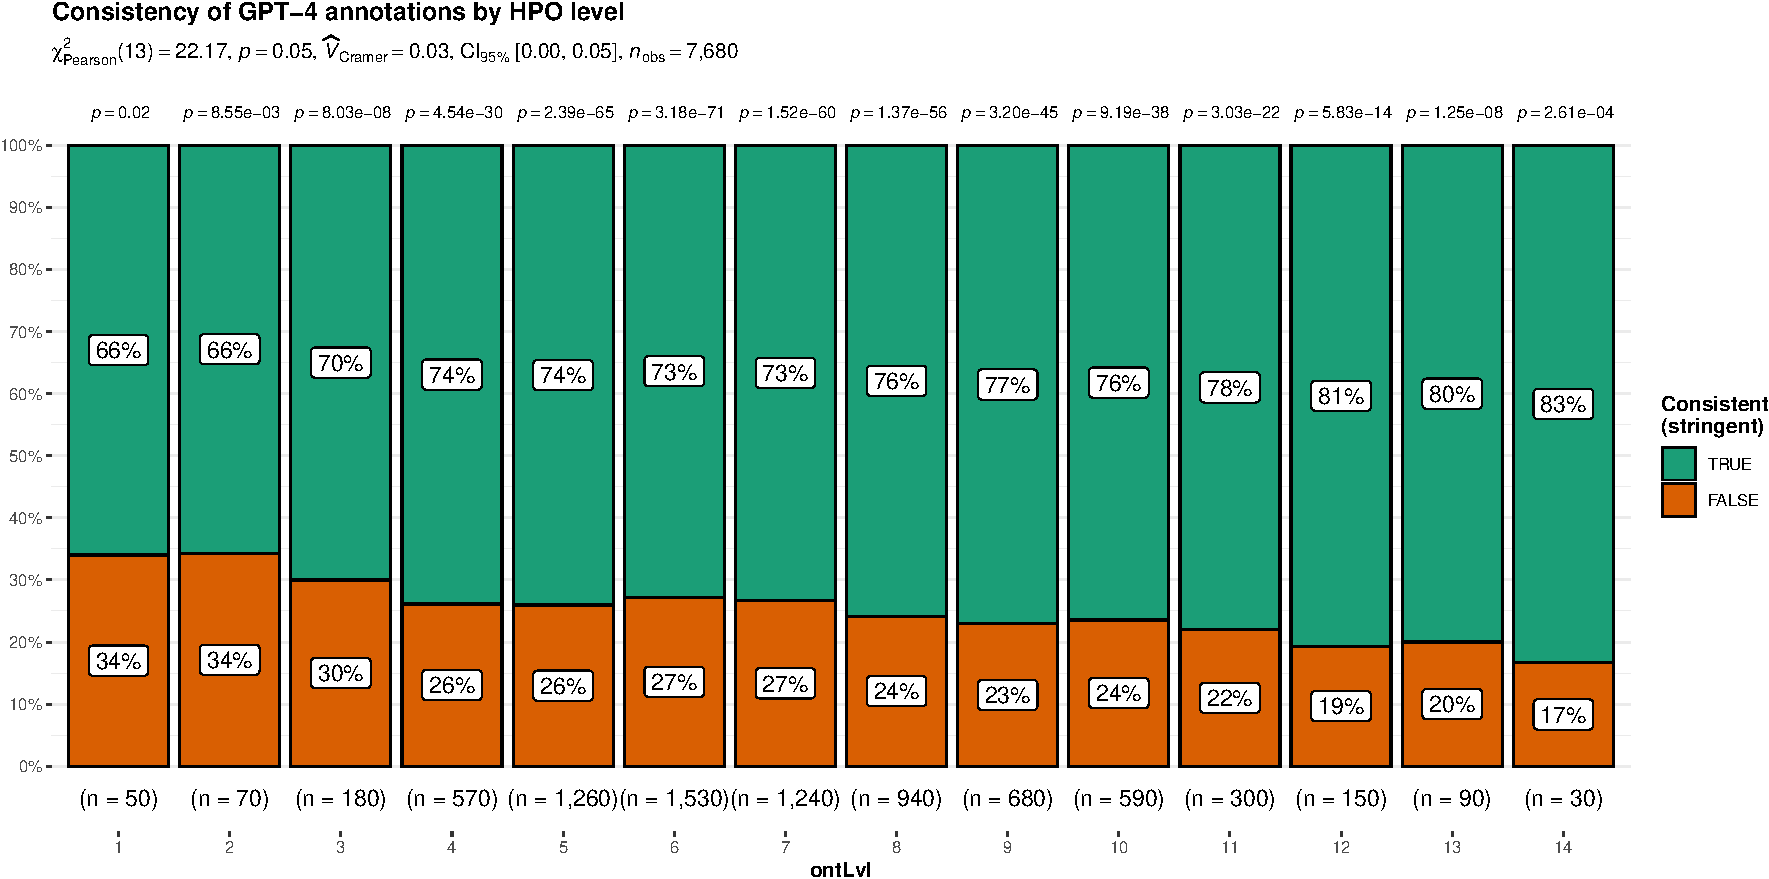
\includegraphics{manuscript_files/figure-pdf/fig-consist-vs-ontLvl-1.pdf}

}

\caption{\label{fig-consist-vs-ontLvl}Relationship between the
consistency of GPT-4 annotations (using the stringent criterion) and the
level of each phenotype within the HPO ontology (with the number of
phenotypes in parentheses). Greater ontology levels (x-axis) indicate
more specific phenotypes. The subtitle indicates summary statistics for
the overall relationship between HPO level and the proportion of
phenotypes that were annotated consistently. The p-values above each bar
indicate whether the distribution of consistent/inconsistent
annotations, within a given HPO level, significantly deviate from the
expected null distribution.}

\end{figure}%

\phantomsection\label{cell-fig-severity-histo}
\begin{figure}[H]

\centering{

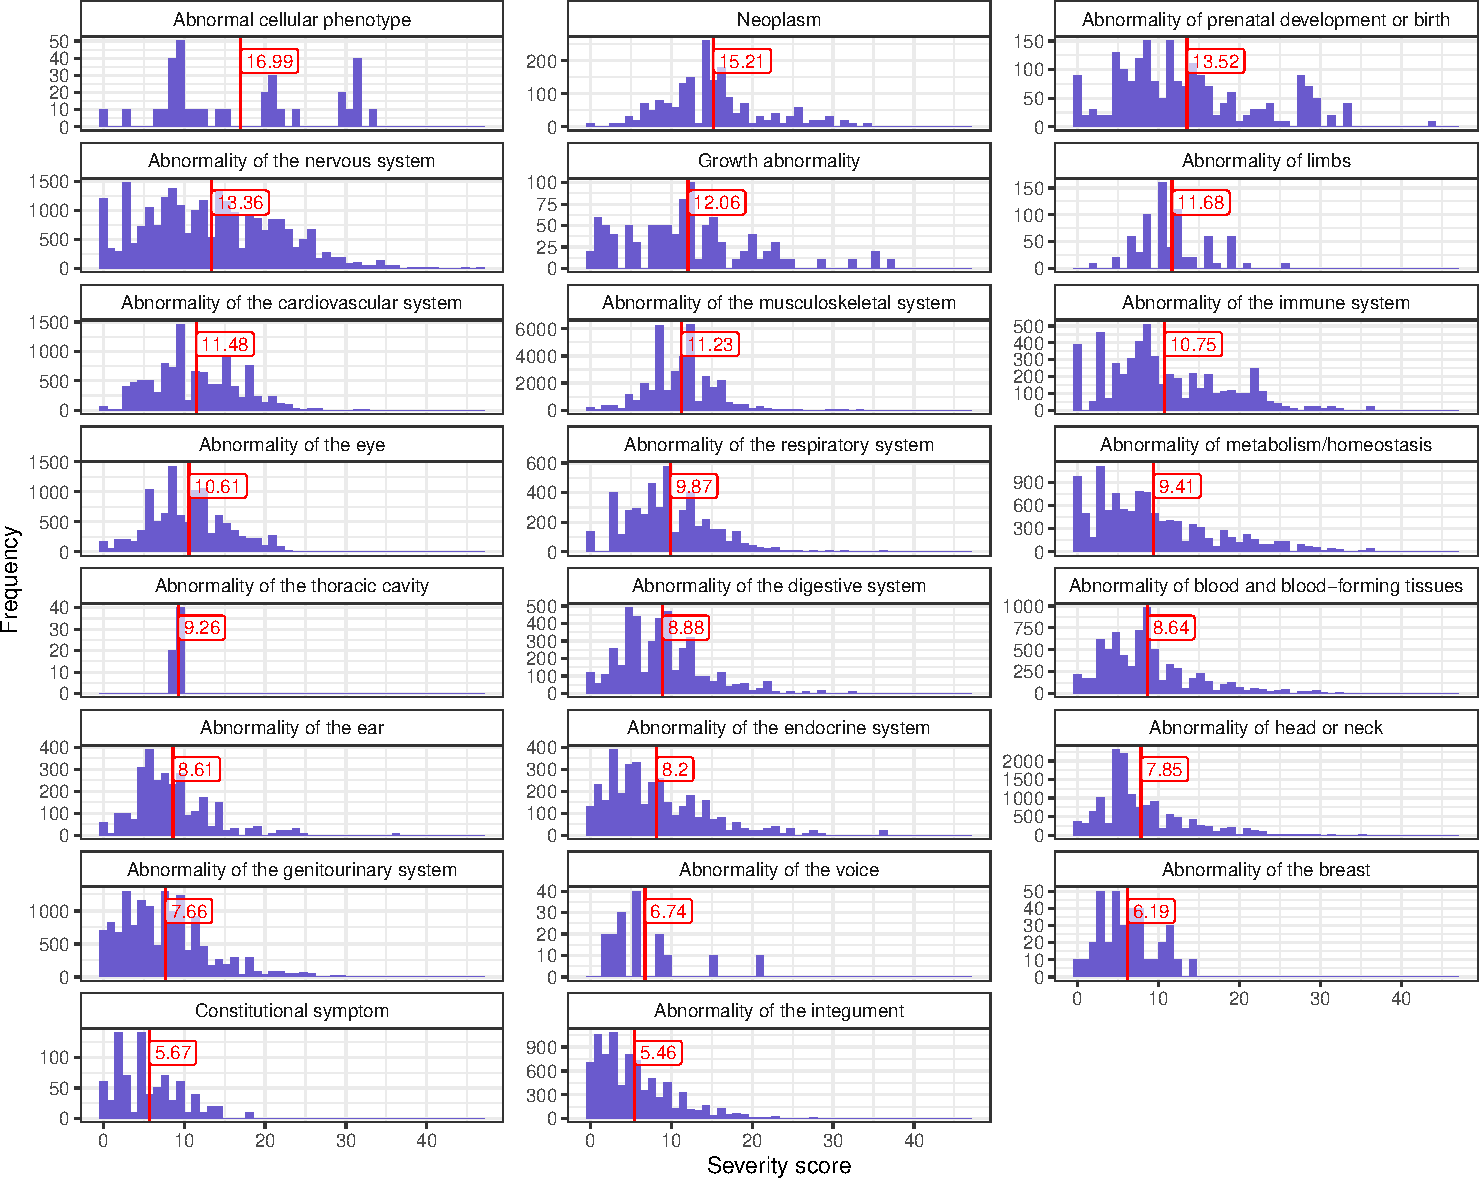
\includegraphics{manuscript_files/figure-pdf/fig-severity-histo-1.pdf}

}

\caption{\label{fig-severity-histo}Distribution of the composite GPT-4
severity score of the severity scores for all HPO terms.}

\end{figure}%

\phantomsection\label{cell-fig-severity-boxplot}
\begin{figure}[H]

\centering{

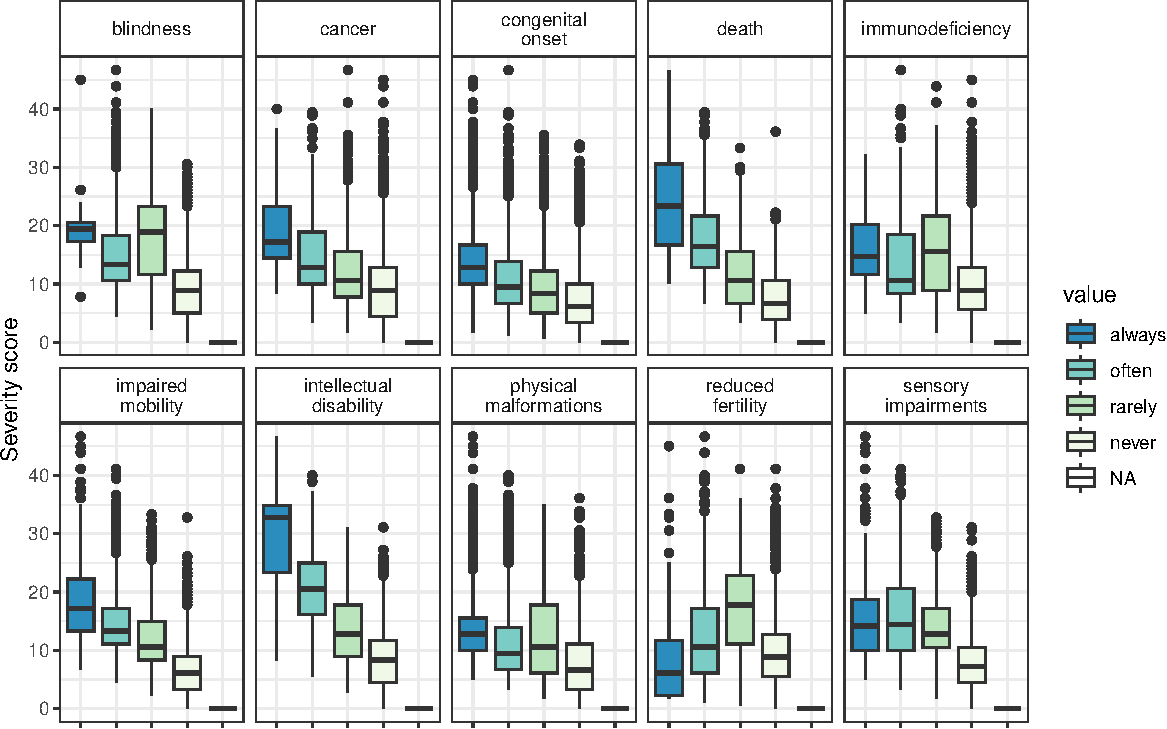
\includegraphics{manuscript_files/figure-pdf/fig-severity-boxplot-1.pdf}

}

\caption{\label{fig-severity-boxplot}Boxplot showing the relationship
between composite severity score (y-axis) and the frequency response
categories within each annotation type.}

\end{figure}%

\phantomsection\label{cell-fig-metric-corplot}
\begin{figure}[H]

\centering{

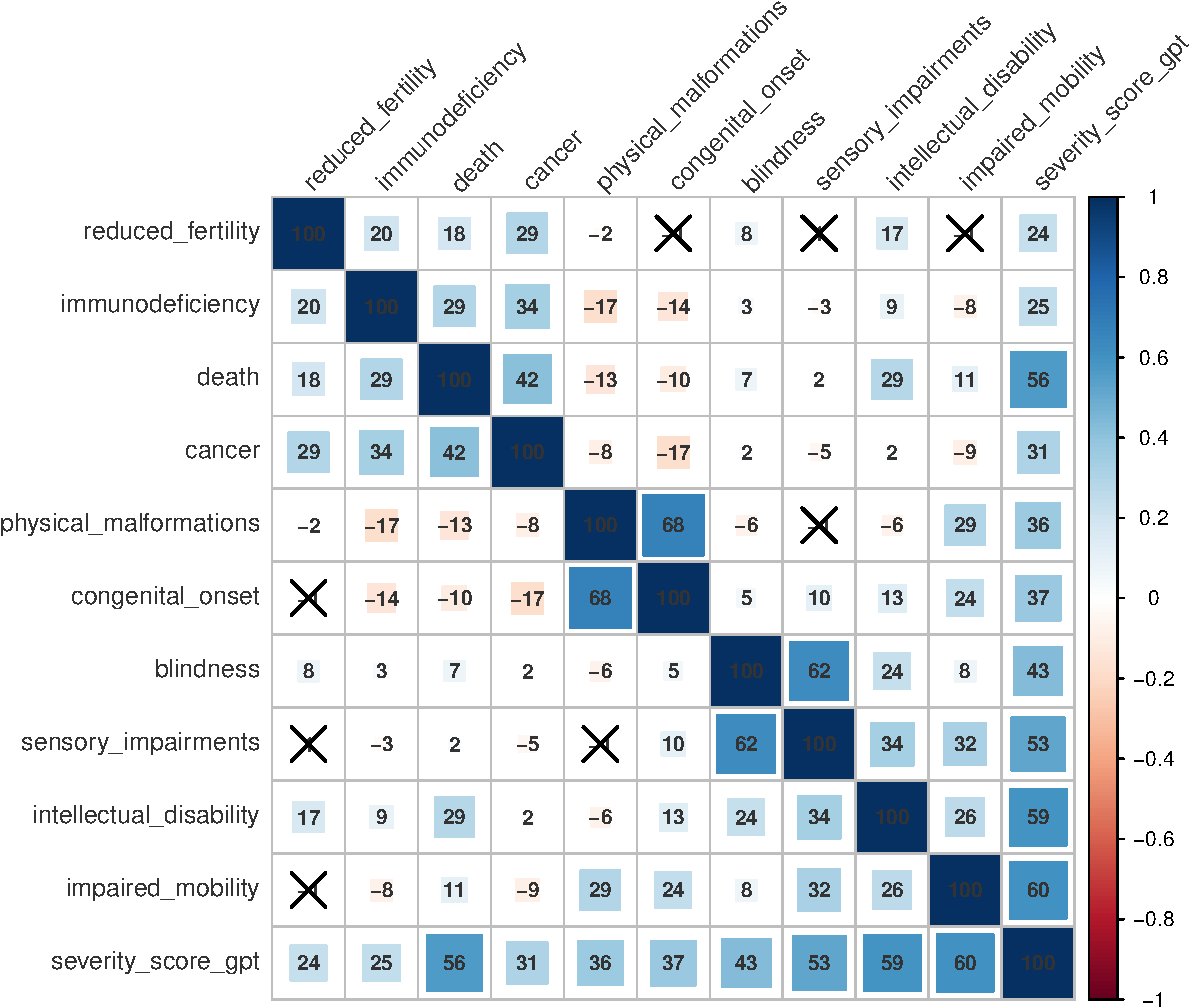
\includegraphics{manuscript_files/figure-pdf/fig-metric-corplot-1.pdf}

}

\caption{\label{fig-metric-corplot}Pearson correlations between each
individual severity metric and the composite severity score
(`severity\_score\_gpt').}

\end{figure}%

\phantomsection\label{cell-fig-severity-class}
\begin{figure}[H]

\centering{

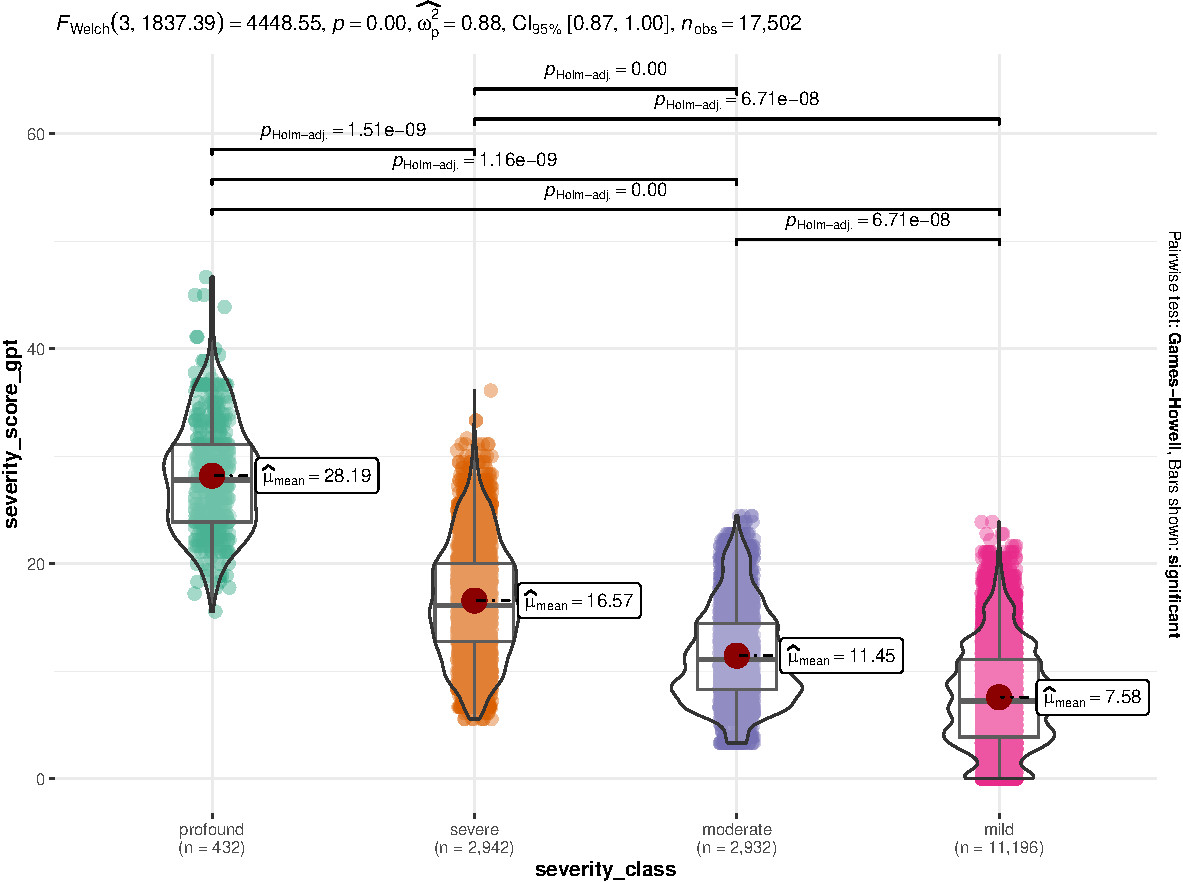
\includegraphics{manuscript_files/figure-pdf/fig-severity-class-1.pdf}

}

\caption{\label{fig-severity-class}Distribution of the composite GPT-4
severity score introduced in this paper (y-axis) by an approximation of
the severity class system introduced Lazarin et al. (2014) (x-axis).
While these are different schemes for ranking phenotype severity, there
is a strong correspondence between them (see summary statistics in
subtitle). The sample size (number of phenotypes) is shown in
parentheses along the x-axis.}

\end{figure}%

\newpage{}

\subsubsection{Supplementary Tables}\label{supplementary-tables}

\begin{table}

\caption{\label{tbl-annotations}Table of GPT-4 annotations for all Human
Phenotype Ontology (HPO) phenotypes in Figure~\ref{fig-top-phenos}. For
each phenotype, this includes the name of the phenotype (`hpo\_name'),
the ID of the phenotype (`hpo\_id'), the frequency of each annotation
(always, often, rarely, never), and the justification for each
annotation ('\ldots\_justification'). These results can also be
downloaded programmatically using the R function
\texttt{HPOExplorer::gpt\_annot\_check}.}

\centering{

\href{https://github.com/neurogenomics/gpt_hpo_annotations/raw/master/data/top_phenos_annotations.csv.gz}{\textbf{Top
phenotype annotations table}}

}

\end{table}%

\begin{longtable}[]{@{}
  >{\raggedright\arraybackslash}p{(\columnwidth - 4\tabcolsep) * \real{0.2000}}
  >{\raggedright\arraybackslash}p{(\columnwidth - 4\tabcolsep) * \real{0.2000}}
  >{\raggedright\arraybackslash}p{(\columnwidth - 4\tabcolsep) * \real{0.6000}}@{}}

\caption{\label{tbl-fas}Severity nnotations generated for GPT-4
annotations for the HPO phenotype `Fetal akinesia sequence'
(HP:000198).}

\tabularnewline

\toprule\noalign{}
\begin{minipage}[b]{\linewidth}\raggedright
Clinical characteristic
\end{minipage} & \begin{minipage}[b]{\linewidth}\raggedright
Annotation
\end{minipage} & \begin{minipage}[b]{\linewidth}\raggedright
Justification
\end{minipage} \\
\midrule\noalign{}
\endhead
\bottomrule\noalign{}
\endlastfoot
Intellectual disability & always & Fetal akinesia sequence typically
results in severe neurodevelopmental impairment, including intellectual
disability. \\
Death & always & Fetal akinesia sequence is typically fatal in utero or
shortly after birth. \\
Impaired mobility & always & Fetal akinesia sequence results in severe
physical impairment, including impaired mobility. \\
Physical malformations & always & Fetal akinesia sequence is associated
with multiple physical malformations. \\
Blindness & often & Visual impairment is common in surviving individuals
with fetal akinesia sequence due to neurodevelopmental impairment. \\
Sensory impairments & always & Fetal akinesia sequence typically results
in severe sensory impairment due to neurodevelopmental disruption. \\
Immunodeficiency & rarely & While not a direct feature, some individuals
with fetal akinesia sequence may have associated immune
abnormalities. \\
Cancer & never & Fetal akinesia sequence does not cause cancer. \\
Reduced fertility & often & Given the severe physical impairments
associated with fetal akinesia sequence, fertility is likely to be
reduced in surviving individuals. \\
Congenital onset & always & Fetal akinesia sequence is a congenital
disorder. \\

\end{longtable}



\end{document}
